\subsection{Log File}

A log is written to a file so that the programmer can retrace the steps in the event of an unexpected program response. This file is overwritten or recreated each time the game is started. In the program, a class Log is created to use a logger object to log messages for a specific system or application component. Furthermore, a simple method "WriteToLog " is created in order to let Class logic implement and conveniently document when an event happens, for example, a player places a token on the board. Furthermore, there is also some situation when the game encounter a problem such as the no Token in the deck and the player could not have a new Token. The representation of the Log File is shown as Figure \ref{fig: logFile} below.

\begin{figure}[h]
	\centering
	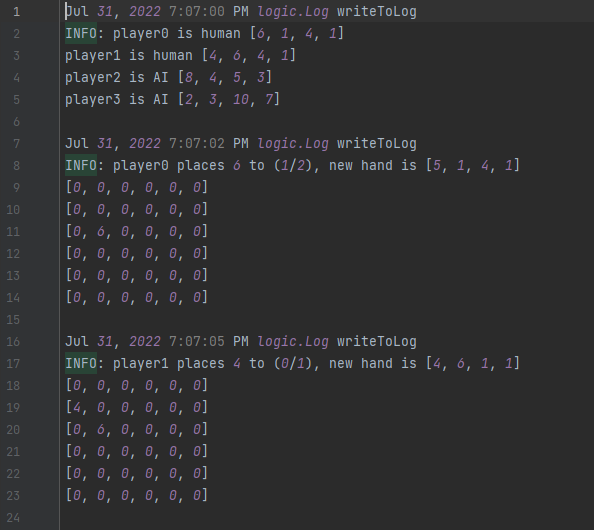
\includegraphics[width=0.8\textwidth]{image/logFile}
	\caption{The representation of Log file}
	\label{fig: logFile}
\end{figure}

